\documentclass{pracamgr}
\usepackage{polski}

\usepackage[utf8]{inputenc}
\usepackage[OT4]{fontenc}

\usepackage[pdftex]{graphicx}
\usepackage{wrapfig}
\usepackage{subfig}
\usepackage{amsmath}
\usepackage{enumerate}
\usepackage{textcomp}
% Dane magistranta:

\author{Małgorzata Habich}

\nralbumu{280454}

%\title{Systemowa analiza reakcji drożdży na szok cieplny}
\title{Globalny metabolizm jako sensor stresu - analiza odpowiedzi na temperaturę u drożdży}

\tytulang{---> tytuł ang <---} %TODO

%kierunek: Matematyka, Informatyka, ...
\kierunek{Bioinformatyka i biologia systemów}

% informatyka - nie okreslamy zakresu (opcja zakomentowana)
% matematyka - zakres moze pozostac nieokreslony,
% a jesli ma byc okreslony dla pracy mgr,
% to przyjmuje jedna z wartosci:
% {metod matematycznych w finansach}
% {metod matematycznych w ubezpieczeniach}
% {matematyki stosowanej}
% {nauczania matematyki}
% Dla pracy licencjackiej mamy natomiast
% mozliwosc wpisania takiej wartosci zakresu:
% {Jednoczesnych Studiow Ekonomiczno--Matematycznych}

% \zakres{Tu wpisac, jesli trzeba, jedna z opcji podanych wyzej}

% Praca wykonana pod kierunkiem:
% (podaæ tytu³/stopieñ imiê i nazwisko opiekuna
% Instytut
% ew. Wydzia³ ew. Uczelnia (je¿eli nie MIM UW))
\opiekun{dra Pawła Szczęsnego\\
  --> INSTYTUT <--- \\%TODO
  }

% miesi±c i~rok:
\date{Czerwiec 2013}

%Podaæ dziedzinê wg klasyfikacji Socrates-Erasmus:
\dziedzina{ 
%11.0 Matematyka, Informatyka:\\ 
%11.1 Matematyka\\ 
%11.2 Statystyka\\ 
%11.3 Informatyka\\ 
%11.4 Sztuczna inteligencja\\ 
%11.5 Nauki aktuarialne\\
11.9 Inne nauki matematyczne i informatyczne
}

%Klasyfikacja tematyczna wedlug AMS (matematyka) lub ACM (informatyka)
\klasyfikacja{--> KLASYFIKACJA <--} %TODO

% S³owa kluczowe:
\keywords{--> SŁOWA KLUCZOWE <-- }%TODO

% Tu jest dobre miejsce na Twoje w³asne makra i~¶rodowiska:
\newtheorem{defi}{Definicja}[section]

% koniec definicji

\begin{document}
\maketitle

%tu idzie streszczenie na strone poczatkowa
\begin{abstract}
--> ABSTRAKT <--
%TODO
\end{abstract}

\tableofcontents
%\listoffigures
%\listoftables

\chapter{Wprowadzenie}

\section{Temperatura jako czynnik stresowy}

Temperatura stanowi uniwersalny czynnik stresowy w świecie komórkowym. Pomijając nieliczne organizmy należące do grupy hipertermofili, wzrost temperatury stanowi poważne zagrożenie
dla prawidłowego funkcjonowania i życia komórki. Dzieje się tak dlatego, że temperatura oddziałuje bezpośrednio na wszystkie elementy systemu zaburzając homeostazę. 
Z punktu widzenia termodynamiki wzrost ciepła wiąże się ze wzmożonym ruchem atomów. W wyniku tego rozrywają się wiązania krótkiego zasięgu (tj. wiązania wodorowe i oddziaływania Van der Waalsa) oraz 
zwiększa się ruchliwość cząsteczek. Złożenie tych dwóch zjawisk ma dla komórki bardzo szerokie skutki.

Jednym z największych problemów z jakimi musi sobie poradzić komórka podczas wzrostu temperatury jest denaturacja białek. Funkcja tych związków wiąże się bezpośrednio z ich kształtem, za który odpowiadają 
wiązania wodorowe podtrzymujące strukturę drugorzędową. Gdy wzrasta temperatura wiązania rozrywają się i najczęściej w sposób nieodwracalny zaburzana jest struktura białka. Denaturacja niesie za sobą
dwa problemy z punktu widzenia komórki. Z jednej strony tracą one niezbędne do funkcjonowania składniki, które trzeba uzupełnić, a z drugiej strony zdenaturowane białka mają tendencję
do agregacji przez co zajmują miejsce i utrudniają swoją degradację. Należy jednak pamiętać, że nie wszystkie białka są równie czułe na temperaturę. Dzięki temu możliwe jest wczesne wykrycie wzrostu temperatury (białka
wyjątkowo czułe) oraz przeżycie podczas warunków stresowych (najcześciej białka które pojawiają się podczas wzrostu temperatury mają budowę bardziej odporną na działanie tego czynnika) \cite{TsInEubact}.

Rozrywanie się wiązań wodorowych niesie ze sobą również inne konsekwencje. Wiązania wodorowe podtrzymują strukturę RNA i DNA. Poprzez działanie temperatury może dochodzić do superskręcania się DNA co uniemożliwia 
ekspresję genów oraz rozklejania się specyficznych struktur RNA. Podobnie jak w przypadku białek część organizmów umie to obrócić na swoją korzyść. W przypadku E.coli system wyczuwania zmian temperatury opiera się
w dużej mierze na różnicach w topnieniu RNA i DNA \cite{TsInEubact, Digel08}.

Innym problemem związanym z rozluźnianiem się wiązań jest zwiększona płynność błony komórkowej. Niestety nie jest to zbyt dobrze zbadany problem \cite{Membranefluidity}, ale obecne wyniki pozwalają zaobserwować zwiększoną
płynność błony komórkowej, rozluźnienie jej struktury, a tym samym większą przepuszczalność. Z uwagi na bardzo groźne konsekwencje dla komórki reakcja systemu jest bardzo szybka i prowadzi do zagęszczenia błony.

Nie tylko rozrywanie się wiazań wodorowych stanowi problem dla komórki. Podwyższenie się temperatury prowadzi do zwiększenia się szybkości reakcji enzymatycznych. Zgodnie z regułą $Q_{10}$ przeciętny wzrost
szybkości reakcji wzrasta dwukrotnie przy zmianie temperatury o 10 \textcelsius, aż do gwałtownego spadku związanego z denaturacją białka. Niekontrolowane zwiększenie się szybkości reakcji enzymatycznych
może prowadzić do nagromadzenia się produktów, nieoptymalnego wydatku energii i zaburzeniu homeostazy. W badaniach przeprowadzonych na bakteriach zaobserwowano między innymi wzrost szybkości glikolizy oraz spadek przepływów przez 
cykl Krebsa \cite{Wittmann07}.

Patrząc na komórkę jako na całość można zaobserwować również wpływ temperatury na jej cykl życiowy. Pod wpływem wielu zmian które następują w komórce w wielu organizmach jednokomórkowych np. drożdżach 
następuje zatrzymanie się w fazie G$_1$.

\section{Reakcja na temperaturę u drożdży}

Optymalna temperatura wzrostu drożdży różni się w zależności od szczepu, ale przyjmuje się, że są to temperatury w 
zakresie między 25 \textcelsius, a 30 \textcelsius. Powyżej 36 \textcelsius\ uruchamiany jest system ochrony komórki
zwany HSP (heat shock response). Maksymalną temperaturą, w której mogą rozwijać się jest 42 \textcelsius\ powyżej której 
następuje inaktywacja polimerazy II RNA \cite{Morano12}.

Tradycyjne doświadczenie polegające na badaniu reakcji drożdży na temperaturę polega na inkubacji komórek w 30 \textcelsius, a
następnie przeniesieniu ich do 37 \textcelsius. Wykonywane były oczywiście również inne dobory parametrów, ponieważ 
reakcja różni się w zależności od czasu ekspozycji na temperaturę, jak często następuje podgrzanie, jak szybko zmieniana
jest temperatura itd.

Już w latach 80' zaobserwowano, że ekspozycja drożdży na działanie temperatury wywołuje pojawienie się białek, których 
wcześniej nie było w proteomie komórki \cite{Miller1979}, a wcześniejsza inkubacja w wyższej temperaturze pozwala 
na uniknięcie śmierci w ekstremalnych warunkach 50 \textcelsius \cite{Mcalister1980}.

Reakcję drożdży na temperaturę można rozpatrywać na kilku poziomach złożności. Patrząc z punktu widzenia makro na komórkę
można zaobserwować zmiany w cyklu życiowym. Organizm poddany szoku termicznemu zatrzymuje się w fazie G$_1$. Dzieje się tak 
z uwagi na redukcję transkryptów, oraz posttranslacyjne modyfikacje cyklin fazy G$_1$/S CLN1 oraz CLN2 \cite{CyclinArrest}. Jest to prawdopodobnie
wywołane nagromadzeniem się zdenaturowanych białek, co pośrednio aktywuje czynnik transkrypcyjny Hsf1 \cite{MisfoldedProteins}. Można się domyślać, że 
podział komórki w niesprzyjających okolicznościach mógłby mieć dla niej katastrofalne skutki.	

Komórki drożdży są ograniczone od świata zewnętrznego poprzez błonę komórkową i ścianę złożoną z glukozo- i maltozo- polisacharydów,
 i N-acetyloglukozoamin. Podczas swojego życia utrzymują one wysokie ciśnienie wewnętrzne sprawiając, że nawet małe defekty w ścianie 
 są potencjalnie letalne. W przestrzeni periplazmatycznej znajduje się wiele pierwotnych receptorów na stres w tym termalny.
 Pod wpływem temperatury uruchamiają się szlaki sygnalizacji komórowej co prowadzi do zwiększonej produkcji $\beta$1,6-glukanu
 oraz białek CWP (cell wall proteins) \cite{CellWall}. Ponadto zmniejsza się ilość nienasyconych kwasów tłuszczowych w błonach \cite{CellLipids}
 dzięki czemu równoważona jest zwiększona płynność błony.
 
 Istotna zmiana następuje w metabolizmie komórki. Mimo, że nie jest znany dokładny mechanizm reakcji komórki na zwiększone 
 tempo reakcji enzymatycznych, to można zaobserwować inne ciekawe zmiany. Największe widać w reakcjach odpowiedzialnych za
 metabolizm cukrów. Pod wpływem podwyższonej temperatury następuje akumulacja glicerolu \cite{GlycerolAccumulate} oraz
 zwiększa się produkcja trehalozy. Dwucukier występuje również w warunkach normalnych w komórce, lecz w blisko sto razy mniejszym stężeniu. 
 Jego zadaniem jest chronić białka przed denaturacją i po obniżeniu temperatury jego poziom wraca do pierwotnego stanu. Inną obserwowaną
 zmianą jest podwyższenie się ilości cAMP. Jest to o tyle interesujące, że poziom tego związku wpływa na aktywację PKA które negatywnie
 reguluje działanie czynnika transkrypcyjnego Msn2/4 odpowiedzialnego za większość reakcji temperaturowych. Prawdopodobnie 
 jest to wewnętrzny hamulec systemu nie pozwalajacy na przesadzoną reakcję na stres \cite{Blomberg00,StressResponse99}.

 Największą przemianą jaka następuje w komórce podczas reakcji na temperaturę jest zmiana profilu białkowego. Za większość tej 
 reakcji odpowiadają czynnki transkrypcyjne Hsf1 i Msn2/4. Przyłączają się one odpowiednio do sekwencji oznaczonych jako 
 HSE (\textbf{H}eat \textbf{s}hock \textbf{e}lements) i oraz STRE (\textbf{st}ress \textbf{r}esponse \textbf{e}lements).
 Wiele białek, które powstają poprzez przyłączenie się do sekwencji HSE
 jest chaperonami odpowiedzialnymi za fałdowanie się białek, transport, dojrzewanie i degadację enzymów. Ponad to, do tej grupy
 należą enzymy ubikwitynujące (np. Ubc4) , chaperoniny (Hsp60), białka towarzyszące i wiele innych. Odpowiedź wynikająca z 
 przyłączenia się Msn2/4 do STRE ma bardziej charakter metaboliczny np. odpowiedzialne za produkcję i degradację trehalozy, 
 alternatywne izoformy białek glikolizy itd. \cite{MsnContraHsf1}. Badania wskazują, że podczas szoku cieplnego może zmieniać się
 ekspresja nawet do 12\% białek \cite{TransciptomeUponHeatShock}.
 
 W każdym  momencie życia komórki setki białek biorą udział w niezliczonych reakcjach w cytozolu. Biorąc pod uwagę ich ekstremalnie
 duże stężenie (ponad 300 mg/ml) oraz ciągły dopływ wynikający z syntezy nowych makromolekuł staje się oczywiste, że 
 kontrola jakości białek jest kluczowym problemem z jakim boryka się komórka podczas szoku cieplnego.
 Typową obserwacją w komórkach wystawionych na wzrost temperatury jest nagromadzenie się źle sfałdowanych białek. 
 W przypadku drożdży taka reakcja pojawia się dopiero przy temperaturach ekstremalnych, powyżej 50 \textcelsius. Można
 wtedy obserwować zarówno toksyczną agregację zdenaturowanych białek jak i groźne dla funkcjonowania komórki ubytki w 
 ilości białek niezbędnych do życia. Podczas umiarkowanego szoku termicznego (ok. 36-37 \textcelsius) nie obserwuje się
 agregatów. Prawdopodobnie wynika to z bardzo sprawnej maszynerii odpowiedzi na stres cieplny, ubikwitynacji zdenaturowanych
 białek i ich degradacji. Największą rolę pełnią w niej chaperony. Chaperony dzielą się na klika 
 rodzin z których każda pełni trochę inną funkcję. Hsp70 odpowiadają za prawidłowe sfałdowanie się dopiero co powstających białek oraz
 refałdowanie zdenaturowanych. Ich rola polega na poprawianiu struktury czwartorzędowej poprzez przykrywanie nieprawidłowo wystawionych fragmentów 
 hydrofobowych pozwalając im schować się do wnętrza białka. Do klasy Hsp70 należą między innymi białka Ssa, Ssb i Sse. W przeciwieństwie do
 Hsp70 chaperony Hsp90 są dużo bardziej wybredne w doborze substratów. Ich funkcja polega na wspomaganiu końcowego składania się kinaz i wielu czynników transkrypcyjnych. 
 Dokładny mechanizm działania i doboru Hsp90 nie jest znany, lecz wiadomo, że polega na swoistym tańcu chaperonu i pomocniczych białek opiekuńczych 
 wymuszających prawidłowe sfałdowanie się substratu. Przykładem takiego substratu jest wcześniej wspominany Hsf1. Kolejną rodziną 
 chaperonów pojawiających się w trakcie szoku cieplnego są Hsp104. Białka te posiadają unikatową wśród eukariotów umiejętność znajdowania
 agregatów białkowych i rozpuszczania ich, kierując zdenaturowane białka na drogę refałdowania. Ostatnią grupą o której warto wspomnieć
 są małe chaperony tzw. sHsp do których należą między innymi Hsp26, Hsp42 oraz Hsp12. Ich rolą jest wspieranie rozpuszczalności i stabilności białek
 podczas szoku cieplnego. Podobną funkcję do chaperonów pełnią chaperoniny, których stężenie również wzrasta podczas niesprzyjających warunków.
 Chaperoniny tworzą podwójnie-pierścieniowe struktury wewnątrz których zwijane są białka z udziałem ATP. Ograniczenie przestrzeni i aktywny udział chaperoninów
 pozwala na sprawne składanie białek niezależnie od warunków środowiska \cite{Bible}.
 % Problemy z DNA i reakcja na temperaturę są oddzielnie kontrolowane \cite{Duallyregulated85}

\section{Sensory reakcji na stres temperaturowy}

W przeciwieństwie do innych czynników stresowych temperatura oddziałuje praktycznie w tym samym czasie na całą komórkę. 
Dzięki temu sensory tego bodźca możemy znaleźć nie tylko w formie białek zwieszonych w błonie komórkowej, ale również 
pod postacią mRNA czułego na temperaturę, białek o niskiej temperaturze denaturacji, czy wreszcie odpowiedzi metabolizmu.

Wydaje się, że pierwszymi sensorami temperatury są białka błonowe które uruchamiają dalsze kaskady sygnalizacyjne. Do 
najlepiej poznanych należy ścieżka aktywacji HOG której receptorem jest białko błonowe Sho1, a końcowym wynikiem 
aktywacja czynników transkrypcyjnych z rodziny Msn \cite{SensingLesson}. Innym często wymienianym w literaturze szlakiem sygnałowym odpowiedzialnym 
za reakcję na temperaturę jest szlak CWI (cell wall integrity) który odpowiada za czynniki traskrypcyjne wspierające 
naprawę ściany komórkowej. \cite{CWI} 
Co ciekawe błona komórkowa nie jest jedynie biernym organellum które chroni
komórkę i służy jako rusztowanie dla sensorów, ale również sama jej płynność stanowi informację dla komórki o szoku cieplnym.
Dynamika błony komórkowej ma wpływ na reakcję HSR \cite{Carratu96}.

Stosunkowo szybką reakcją jest sposób sygnalizacji wynikający z nagromadzenia się zdenaturowanych białek. Dzięki tej ścieżce
sygnałowej aktywowany jest czynnik transkrypcyjny Hsf1 - najbardziej charakterystyczny wyznacznik szoku cieplnego. Dokładny mechanizm
sygnalizacji jest jednak niejasny i w sposób bardziej szczegółowy przedstawie go w dalszej części pracy.

Kolejnym typem sygnalizacji są termometry RNA. Jest to co prawda bardziej wtórny sposób sygnalizacji, ponieważ dotyczy się
transkryptów białek które mają dopiero powstać, lecz wpływa ona również na kształtowanie się odpowiedzi komórki na stres cieplny.
Jak wynika z badań białka o kluczowej roli dla reakcji na szok temperaturowy mają wyższą temperaturę topnienia mRNA, natomiast białka 
których ekspresja się zmniejsza mają niższą. Ponad to zaobserwowano, że białka pojawiające się pod wpływem czynników transktypcyjnych Msn2/4
charakteryzują się większą stabilnością niż inne białka \cite{RNAterm,Roca11}.

W literaturze nie ma danych na temat białek w Saccharomyces cerevisiae działających jak tradycyjne termometry proteinowe. Czasami
wspomina się o Hsp70 jako białku który pełni taką funkcję \cite{Hsp70thermometer}. Rzeczywiście, z uwagi na jego wiązanie się z czynnikiem transkrypcyjnym Hsf1
wpływa na transkrypcje białek odpowiedzi na szok cieplny, ale nie jest to oparte na jego własnej denaturacji.

Nieznane są globalne sensory zmian w metabolizmie jednak systemom udaje się utrzymać homeostazę. Jak pokazno 
na przykładzie glikolizy za stabilizację reakcji enzymatycznych mogą odpowiadać systemy autokatalityczne i 
inne struktury topologiczne czułe na wzrost temperatury \cite{Mair05,AutocatalysisGlycolysis} 

%TODO glikolza
% 
% 
% 
% The Response to Heat Shock and Oxidative Stress
% in Saccharomyces cerevisiae \cite{Morano12}


% 
%   Glikoliza Control of Glycolytic Oscillations by Temperautr Mair et all




\chapter{Cel pracy}

Celem pracy jest stworzenie możliwie pełnego systemu wykrywania wzrostu temperatury przez drożdże. 
Jak dotąd pojawiło się wiele prac które w oderwaniu od siebie wskazywały na możliwość pobudzenia
temperaturowego danego szlaku sygnalizacyjnego, lecz nie udało mi się znaleźć takiej która by 
zbierała obecnie dostępną wiedzę na ten temat. Z uwagi na to, że obecne prace skupiają się
przede wszystkim na pojedynczych szlakach sygnalizacyjnych, to brakuje badań na temat 
interakcji szlaków ze sobą i połączeń między nimi które próbowałam znaleźć. Ponad to warto zwrócić uwagę, że
nie istnieją obecnie wyniki które by wskazywały na to jaki jest wkład przesunięć metabolicznych
komórki w systemy sygnalizacji szoku cieplnego. Na podstawie glikolizy zbadałam reakcje ciągu 
enzymatycznego na wzrost wartości km białek. Cała moja praca może służyć jako wstęp do dalszych badań
nad reakcją drożdży na szok cieplny, a szczególnie nad próbą oszacowania ilościowego wkładu 
wzrostu szybkości reakcji enzymatycznych na całość procesów zachodzących w komórce podczas szoku terminczego.

Badania nad reakcją drożdży na temperaturę są istotne z uwagi na trzy podstawowe aspekty. Po pierwsze 
mają one znaczenie przemysłowe - od tysięcy lat drożdże towarzyszą ludzkości jako organizmy 
produkujące alkohol oraz wykorzystywane do celów piekarskich. Gdy w 1857 roku Pasteur 
zaprezentował dowód, że to właśnie one odpowiadają za proces fermentacji, ich wykorzystanie 
stało się bardziej świadome, a produkcja alkoholu zaczęła być optymalizowana 
pod względem wydajnościowym drożdży \cite{100years}. Jak wskazują badania najlepsze rezultaty 
uzyskuje się balansując na wąskiej granicy szoku środowiskowego \cite{Stresstolerance}. Odkrycie i usystematyzowanie wiedzy 
jak drożdże wykrywają wzrost temperatury może mieć znaczące dla rozwoju przemysłu alkoholowego. 
Drugim równie ważnym powodem, jest wykorzystanie drożdża jako organizmu modelowego. Poznanie dokładnych mechanizmów
jakie zachodzą podczas szoku cieplnego może pomóc nam zrozumieć jak to przebiega u innych organizmów. Ostatnim, lecz 
nie najmniej ważnym argumentem za takimi badaniami jest patogeniczność niektórych szczepów drożdży. 
Podwyższenie temperatury jest typą reakcją organizmu na zapalenie. Poznając mechanizmy w jaki sposób 
drożdże wykrywają podwyższenie się temperatury możemy projektować leki uderzające w ten system, a tym samym
uniemożliwiające im dostosowanie się do nowych warunków i w rezultacie powodujące ich śmierć \cite{Drugs}.



% Znaczenie drozdzy \cite{100years}
% Tolerancja na stres kluczowa dla produkcji drozdzy \cite{Stresstolerance}


% Inny model \cite{OtherModel}
% 
% Probuje zobaczyc jaka jest dokladna droga sygnalizacji temperatury. po pierwsze sa bialka blonowe ktore sa dobrze opisane ale ja to zrobilam lepiej
% po drugie sa reakcje bialek po trzecie jest rna po czwarte jest odpowiedz z metabolizmu. generalnie odpowiedz metaboolizmu jest kompenosowana ale pytanie w jaki sposob.
% sa uklady autokatalityczne ktore sa wrazliwe na wahania temperatury. a co ze statystyczna zmiana szybkosci reakcji wynikajacych ze zmiany km od temperatury?
% nikt tego wczesniej nie ruszal wiec aby opracowac pelny model sygnalizacji (bo z pewnoscia metabolizm od razu reaguje) trzeba zajac sie tym.
% nie ma oczywistego sensora w ujeciu komorkowym przesuniec metabolicznych wywolywanych zmianami km/T
% integrancja sensora z reszta systemu

\chapter{Materiały i Metody}
\section{Budowa modelu}

Do budowy modelu korzystałam z progamu Cell Designer dostępnego na stronie www.celldesigner.org w wersji 4.3 . Dane do
modelu czerpałam z dostępnej literatury.

! dane z temperatury 

\section{Badanie właściwości glikolizy}

Do badania właściwości glikolizy korzystałam z programu Copasi dostępnego na stronie  http://www.copasi.org/ w wersji 4.8 .
Jako przykładowy model glikolizy wybrałam model z 2001 roku opublikowany na stronie http://www.ebi.ac.uk/biomodels-main/BIOMD0000000061
oraz opisany w publikacji `Full-scale model of glycolysis in Saccharomyces cerevisiae.' przez Hynne F, Danø S, Sørensen PG. w Biophys. Chem. 2001 Dec; 94(1-2): 121-163.
Zmiany wartości Km oparłam na %TODO 

\section{Poszukiwanie białkowych termometrów}

Dane na temat zakresu odporności na temperaturę pobrałam z bazy danych BRENDA (http://www.brenda-enzymes.info/). Mapowanie na szlaki
metaboliczne umożliwił mi serwis Kegg (http://www.genome.jp/kegg/).


\chapter{Wyniki i dyskusja}
\section{Budowa modelu}
\subsection{Szlak HOG}
\subsubsection{HOG}

\begin{wrapfigure}{r}{0.5\linewidth}
\centering
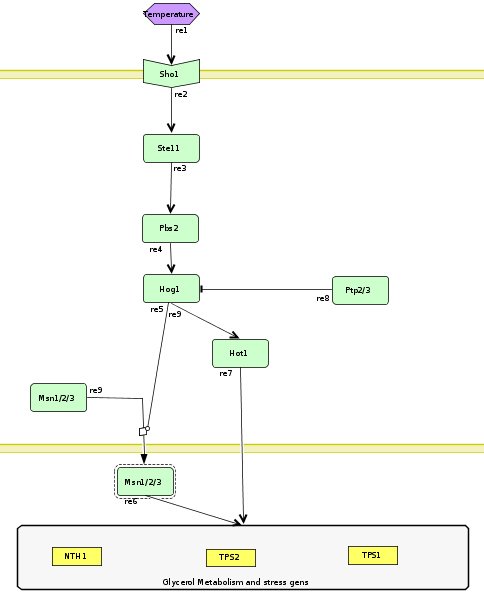
\includegraphics[width=0.4\textwidth]{Obrazy/HOG.png}

\caption{}

\label{fig:myfig}
\end{wrapfigure}

Mimo, że nazwa szlaku HOG wzięła się od szoku osmotycznego (high-osmolarity glycerol) który początkowo
wydawał się jedynym bodźcem pobudzającym pierwotne receptory, obecnie wiadomo, że jest to najbardziej
uniwersalny szlak sygnałowy w komórce. Jego końcowe transmitery będące czynnikami transkrypcyjnymi odpowiadają
za szerokie przygotowanie komórki do wszelkiego rodzaju warunków stresowych.

Szlak HOG w warunkach szoku cieplnego jest pobudzany przez białko błonowe Sho1, początkowo identyfikowane 
jako osmosensor. Nie jest to jedyny możliwy aktywator tego szlaku, ale wydaje się, że inne białka 
nie uczestniczą w aktywacji podczas szoku cieplnego. Prawdopodobnie różne aktywatory pomagają rozróżniać
sygnały pochodzące od innych bodźców i pomagać regulować odpowiedź. Nie jest znany dokładny mechanizm
pobudzenia Sho1.




% The yeast high-osmolarity glycerol (HOG) mitogen-activated protein kinase (MAPK) pathway has been
% characterized as being activated solely by osmotic stress. In this work, we show that the Hog1 MAPK is also
% activated by heat stress and that Sho1, previously identified as a membrane-bound osmosensor, is required for
% heat stress activation of Hog1. The two-component signaling protein, Sln1, the second osmosensor in the HOG
% pathway, was not involved in heat stress activation of Hog1, suggesting that the Sho1 and Sln1 sensors
% discriminate between stresses\cite{Winkler02}
% 
% It was also found that protein tyrosine phosphatases (PTPs) Ptp2 and Ptp3, which inactivate Hog1, have two
% functions during heat stress. First, they are essential for survival at elevated temperatures, preventing lethality
% due to Hog1 hyperactivation. Second, they block inappropriate cross talk between the HOG and the cell wall
% integrity MAPK pathways, suggesting that PTPs are important for maintaining specificity in MAPK signaling
% pathways.\cite{Winkler02}

\subsubsection{Msn2/4}
Two nutrient-sensing pathways have
been described to play important regulatory roles in controlling
Msn2/4: the cAMP-protein kinase A (PKA) pathway and the TOR
pathway\cite{Bible}

As a result, we believe that such
regulons, consisting of fluctuation-correlated genes, reflect biologically
relevant modular structures that might exist to maintain
useful but controlled diversity across a population. Such a bethedging
strategy might be instrumental in allowing a population
of cells to successfully navigate unanticipated changes in its
environment (Thattai and van Oudenaarden, 2004). A scheme
based on a coherently fluctuating program, rather than on a
set of discordantly fluctuating individual genes, would constitute
a robust implementation of a successful bet-hedging program.
The noise regulons we have identified, which are coherently
coordinated within one cell but variable across a population,
might represent such a scenario. In particular, it is interesting
to note the presence of the MSN2/4 pathway, which promotes
survival in the face of acute stress as one such noise regulon.
It is also interesting to note the absence of programs (e.g., an
HSF1 regulon) that mediate long-term adaption and recovery
from stress (Yamamoto et al., 2008). \cite{CellularNoice}

Recent studies showed that Yak1 may contribute to the PKA-dependent inhibition of Msn2/4\cite{Bible}

\subsection{Szalak CWI}
The CWI pathway is activated by heat
through an unknown mechanism that requires at least one member of the putative sensors Mid2 and Wsc1 to Wsc4. In the absence
of these proteins, the HSR is activated normally, but cells are heat
shock sensitive, are autolytic, and do not activate the CWI transcription factor Rlm1\cite{Bible}

Signals are initiated at the plasma
membrane (PM) through the cell surface sensors Wsc1, -2, and -3,
Mid2, and Mtl1. The extracellular domains of these proteins are highly
O-mannosylated. Together with PI4,5P2, which recruits the Rom1/2
GEFs to the plasma membrane, the sensors stimulate nucleotide
exchange on Rho1. Relative input of each sensor is indicated by the
width of the arrows. Rho1 activates five effectors, including the 
Pkc1-MAP kinase cascade, the 1,3-glucan synthase (GS), the Bni1 formin
protein, the exocyst component Sec3, and the Skn7 transcription 
factor. Additional regulatory inputs from the Tus1 GEF, the inhibitory
Rho1 GAPs, and the Pkh1/2 protein kinases are indicated. Pkh1/2 are
activated by phytosphingosine (PHS). The MAP kinase cascade, which
is comprised of Bck1, Mkk1/2, and Mpk1, is activated by Pkc1. Several
MAP kinase phosphatases downregulate Mpk1. Two transcription 
factors, Rlm1 and the SBF complex (Swi4/Swi6), are targets of the MAP
kinase.\cite{CWI}

The Ptp2 and Ptp3 tyrosine phosphatases, which have been
shown to dephosphorylate the Fus3 and Hog1 MAP kinases,
also act on Mpk1 in vivo and in vitro. Both genetic and
biochemical evidence suggests that Ptp2 is more effective than
Ptp3 against activated Mpk1. Additionally, expression of PTP2
but not PTP3 is induced in response to mild heat shock in an
Mpk1-dependent manner, suggesting that activation of Mpk1
establishes a negative feedback loop for its inactivation by
Ptp2. Induction of PTP2 expression is partially under 
the control of Rlm1. The positive regulation of PTP2 expression
by Mpk1 is in contrast to its negative regulation of Msg5
activity. Perhaps Ptp2 and Ptp3 function to reestablish the
resting state of Mpk1 after stress-induced activation.\cite{CWI}

Mpk1 is activated both by cell wall stress and periodically through the cell cycle.
Swi6 is the regulatory subunit that complexes with Swi4 to form SBF,
a cell cycle-specific transcription factor. During periods other than G1,
Swi6 is phosphorylated on Ser160, which causes its exclusion from the
nucleus. It is likely that this phosphorylation is catalyzed by Mpk1. Mpk1
also phosphorylates Swi6 in response to cell wall stress. Swi4, the DNA-
binding component of SBF, associates with Mpk1 in vitro and may
form an alternative transcriptional complex for the regulation of some
cell wall- and morphogenesis-related genes, notably FKS2 and PCL1.\cite{CWI}


\subsection{Szlak Ca$^{2+}$}
Saccharomyces cerevisiae possesses a
high-affinity Ca$^{2+}$ influx system in its plasma membrane comprised of at least two subunits, Cch1 and Mid1. 
Activation of the Cch1-Mid1 channel
results in accumulation of intracellular Ca$^{2+}$ and activation of
calcineurin, the Ca$^{2+}$ and calmodulin-dependent serine/threonine-specific
protein phosphatase. Stimuli that cause activation of Cch1-Mid1
and calcineurin include pheromone treatment, {\bf mild heat shock}, hypoosmotic shock,
endoplasmic reticulum stress, and an increase in extracellular cations (i.e., Li$^+$ and Na$^+$).
Calcineurin dephosphorylates several targets, including the
Crz1/Tcn1 transcription factor, which allows entry of
this factor into the nucleus. Calcineurin also inhibits the
Cch1/Mid1 channel in what appears to be a negative feedback
loop. Recent evidence indicates that a target of
calcineurin action is the Cch1 subunit. Moreover, a screen
of protein kinase knockout mutants revealed that Mpk1 is
required for activation of the Cch1-Mid1 channel in response
to endoplasmic reticulum stress (which may cause cell wall
stress indirectly), suggesting that calcineurin antagonizes CWI
signaling in this instance. It will be interesting to determine
if agents that specifically induce cell wall stress result in
phosphorylation and activation of the Cch1/Mid1 channel. If
so, there exist at least three points of interaction between the
CWI signaling pathway and Ca$^{2+}$ signaling: activation of the
Cch1/Mid1 channel by Mpk1, activation of Crz1 by Rho1-Skn7,
and collaboration between Mpk1 and Crz1 to activate
FKS2 expression in response to cell wall stress.\cite{CWI}


We propose that Crz1 destabilizes Msn2/Msn4 in the nuclei of cells in response to Ca2+ signalling.
One possible physiological interpretation of the CDMD (Crz1-dependent Msn2/4 degradation) is that it minimizes unnecessary
Hog1–Msn2/Msn4-dependent osmotic responses induced by Ca2+ by destabilizing Msn2/Msn4 through Crz1.\cite{Crz1DestabilizesMsn}

Activation of Mpk1 results in
stimulation of Rlm1 and Swi4 transcription factors to drive 
transcription of FKS2 (and other cell wall-related genes) and the Mid1-Cch1
Ca2+ channel. Channel activation leads to stimulation of the Ca2+-
calmodulin-dependent protein phosphatase calcineurin. 
Dephosphorylation of the Crz1 transcription factor by calcineurin allows its entry
into the nucleus. Rho1 may activate the Skn7 transcription factor,
which drives both expression of the OCH1 gene and
stabilization of the Crz1 transcription factor for induction of FKS2.
Thus, CWI signaling and Ca2+ signaling coordinately regulate
expression of the GS-encoding FKS2 gene at several levels.\cite{CWI}
\subsection{Szlak aktywacji Hsf1 i regulacja odpowiedzi za pomocą PKA}
\subsubsection{Hsf1}
Hsf1 is also thought to be negatively regulated
through interactions with several heat shock proteins, including
Hsp82 and members of the Hsp70 family, under both
constitutive and heat shock conditions. To
date, no specific signal that positively regulates Hsf1 activity
during a heat shock has been identified.\cite{TrehaloseRegulatorHsf}

These properties
strongly suggest that the Hsf1 function is modulated largely post-translationally. 
In addition, the loss of two potential control
nodes—nuclear translocation and trimerization—suggests that
the derepression/activation of the Hsf1 transactivation domains is
a plausible regulatory mechanism.\cite{Bible}

 Moreover, a detailed kinetic study 
 demonstrated that Hsf1 is rapidly phosphorylated after heat shock,
declining to a low degree of phosphorylation coincident with the
transient induction of HSP genes. Interestingly, the 
phosphorylation induced by menadione, a pro-oxidant that generates
a superoxide anion in vivo, displays a different and sustained 
kinetic pattern. The two-dimensional resolution of tryptic
phosphopeptides also showed that Hsf1 is phosphorylated at different
phosphor-acceptor sites in response to heat or menadione,
suggesting that Hsf1 undergoes stress-specific phosphorylation.
Although hyperphosphorylation generally correlates with the
transactivation of Hsf1, many phosphorylation events have been
established to repress its transcriptional activity. Sorger first
reported that yeast Hsf1 remains hyperphosphorylated after
the termination of the transient activation of the heat shock response\cite{Bible}


The current model for how cells sense heat shock is as follows.
Heat shock is proposed to cause
the thermal misfolding of a fraction of cellular protein. Because
activation of heat shock factor requires protein synthesis, it is
thought that nascent proteins are the most susceptible to 
thermal denaturation. Misfolded proteins then bind to cytoplasmic
Hsp70 chaperones. Prior to heat shock, these chaperones are
believed to equilibrate between being bound to heat shock
factor (and inactivating it) and being free in the cytoplasm.
Because misfolded proteins bind Hsp70 chaperones very
tightly, their accumulation upon heat shock is proposed to
titrate Hsp70 chaperones, resulting in liberated and active
heat shock factor.\cite{MisfoldedProteins}

\subsubsection{PKA}
The Ras/cAMP/PKA signalling
pathway cAMP had a negative effect on the induction
of the Msn2p/Msn4p regulon, but did not affect the
Hsf1p regulon.\cite{MsnContraHsf1}

Rlm1p appears to be a downstream substrate of the cell integrity pathway MAPK Slt2p.
Rlm1p is a substrate for the MAPK in vitro and shows heat stress-induced, SLT2-dependent phosphorylation
in vivo . Rlm1p also interacts with Slt2p in the two-hybrid system\cite{MAPKinasePathways}

Therefore, we conclude from these studies that PKA antagonizes calcineurin signaling by phosphorylating the Crz1p NLS and thus inhibiting Crz1p nuclear import.\cite{PKAandCalcineurin}

We have found that the guanine nucleotide exchange factor for ras, Cdc25p, interacts with Ssa1p in Saccharomyces cerevisiae.
This interaction was observed with GST-fused Cdc25p polypeptides and confirmed by coimmunoprecipitation with the endogenous Cdc25p.
Hsp82 appeared also to be co-immunoprecipitated with Cdc25p, albeit to a lower level than Hsp70. In a strain deleted for SSA1 and SSA2,
we observed a reduced cellular content of Cdc25p. Consistent with a reduced activity of the cAMP-dependent PKA pathway, the rate of accumulation
of both trehalose and glycogen was stimulated in the ssa-deleted strain. Expression of SSA1 reversed these effects, whereas co-expression of SSA1
and PDE2 restored high accumulation. The expression of genes repressed by cAMP, GAC1 and TPS1, fused to beta-galactosidase, was also stimulated by 
deletion of SSA genes. The effect of ssa deletion on glycogen accumulation was lost in a strain deleted for CDC25 rescued by the RAS2ile152 allele.
Altogether, these results lead to the conclusion that Ssa1p positively controls the cAMP pathway through Cdc25p. We propose that this connection plays
a critical role in the adaptation of cells to stress conditions.\cite{Ssa1ControlscAmp}
\subsection{Trehaloza i glikoliza}

Extensive alteration of gene expression and metabolic remodeling enable the budding yeast Saccharomyces cerevisiae to
ensure cellular homeostasis and adaptation to heat shock. The response logic of the cells to heat shock is still not entirely clear. 
In this study, we combined the expression profiles with metabolic pathways to investigate the logical relations between heat shock response metabolic pathways. 
The results showed that the heat-stressed S. cerevisiae cell accumulated trehalose and glycogen, which protect cellular proteins against denaturation, and modulate 
its phospholipid structure to sustain stability of the cell wall. The TCA cycle was enhanced, and the heat shock-induced turnover of amino acids
and nucleotides served to meet the extra energy requirement due to heat-induced protein metabolism and modification. The enhanced respiration led
to oxidative stress, and subsequently induced the aldehyde detoxification system. These results indicated that new insight into the response logic
of S. cerevisiae to heat shock can be gained by integrating expression profiles and the logical relations between heat shock response metabolic pathways.\cite{ResponseLogic}
\subsubsection{Glycolysis}

One function of this futile cycling
of trehalose may be to increase the intracellular level of
trehalose-6-phosphate, which is a potent inhibitor of the
main hexokinase Hxk2p. This enzyme could be replaced by the Glk1p
and Hxk1p hexokinases, which are induced under heat
shock conditions (this work) and are, respectively, not and
less inhibited by trehalose-6-phosphate. This replacement may have a role in the control of
glycolytic flux and/or alternative pathways (trehalose cycle
and pentose phosphate pathway).\cite{MsnContraHsf1}

A connection between accumulation of intracellular
glycerol and cell-wall-damaging treatments has been
described previously (Garcia-Rodriguez et al., 2000).
Furthermore, our group has postulated a ‘protective
function’ for glycerol besides its role as osmolyte in high
osmotic stress conditions. This may explain why glycerol
is accumulated when cells are shifted to 37 C \cite{GlycerolAccumulate}

\subsubsection{Trehalose}
Such a mechanism can be inferred very nicely from the case of trehalose. Here, the
producing enzymes (trehalose 6-phosphate synthase and phosphatase; Tps1p and Tps2p) have activity
optima at temperatures of 35–45 C, whereas the degrading enzyme (trehalase; Nth1p) has its optimum
temperature at 30 C . With this discrepancy in optimal temperatures, very little trehalose is
produced at 30 C, and because trehalase is at its maximum activity, no trehalose accumulates.
However, at 40 C, trehalose production is high and the trehalase activity is reduced by a factor of
~2.4, which causes trehalose to accumulate. Once the temperature returns to normal values, the direct
temperature dependence of these enzyme activities allows the cell immediately to degrade all trehalose
accumulated at the higher temperature. Not to be wasteful, this degraded trehalose enters glycolysis in
the form of two molecules of glucose.
In a slightly different mechanism, glycogen production and degradation are regulated by cAMP
dependent phosphorylation: in the presence of glucose, glycogen synthase is activated and glycogen
phosphorylase is inactivated; at higher temperatures (35 C), the glucose effects on these enzymes are
amplified.\cite{OtherModel}


The enzymes catalysing the synthesis of trehalose
are localized to the yeast cytosol, where production of the sugar occurs in two steps: first
the glucose moiety from uridine-diphosphate–glucose
is joined to glucose-6-phosphate, forming trehalose-6-phosphate;
the phosphate group is then removed to
yield trehalose and recycle free inorganic phosphate.
The enzymatic complex that carries out this process
consists of at least three distinct, copurifying components
– Tps1p, Tps2p and Tsl1p. A fourth
protein, Tps3p (identified by sequence homology with
Tsl1p), has also been found to associate with Tps1p and
Tps2p (S. Hohmann, pers. commun.). Tps1p catalyses
the first step in trehalose synthesis; cells lacking this
gene produce neither trehalose nor trehalose-6-phosphate.
Phosphatase activity resides in Tps2p;
tps2 mutants accumulate large quantities of 
trehalose-6-phosphate under circumstances in which trehalose
would normally be found. The functions of Tsl1p and
Tps3p are less clear, but these proteins seem to 
contribute to regulation: either gene can be deleted 
without affecting the heat-induced accumulation of 
trehalose by log-phase cells, but accumulation is severely
impaired if both Tsl1p and Tps3p are absent \cite{YinYangTrehalose}


Some previous workers seeking to understand the
mechanism by which heat shock induced the 
accumulation of trehalose argued that the induction of 
expression of TPSZ was an essential key in this process
(Hottiger et al., 1987; Bell et al., 1992), while others
suggested that this rapid accumulation primarily resulted
from the direct effect of temperature on the kinetic
properties of Tre6P synthase complex and trehalase.
Here, we showed that both gene induction and
temperature modulation of kinetic properties of 
trehalose enzymes takes part in this process, but their
relative involvement is strongly linked to the 
temperature range at which heat shocks are performed. Within
temperature upshifts between 33 and 37 "C, the 
transcriptional activation of TPSZ was needed to allow a net,
but otherwise transient, accumulation of trehalose.
Between 37 and 40"C, small changes in the absolute
temperature resulted in a strong reduction of TPSZ
expression, but in great changes of kinetic properties of
Tre6P synthase/phosphatase complex and trehalase. \cite{Parrou97}

In the yeast Saccharomyces cerevisiae, trehalose levels vary
depending on the environment of the cell. The levels are 
almost undetectable during normal exponential growth. After
heat shock, trehalose levels increase rapidly and dramatically,
along with the accumulation of heat shock proteins (HSPs).
This rapid increase in trehalose has been attributed to
the increase in both the translation of the genes involved in the
synthesis of trehalose (TPS1 and TPS2) and the
substrates required for trehalose synthesis. High trehalose levels can stabilize enzymatic
activity and can prevent the aggregation of exogenous proteins
in vivo during heat shock. Trehalose is degraded in the
cytoplasm by neutral trehalase, encoded by the gene NTH1. The transcription of NTH1 is stress responsive;
however, the activity of Nth1 is greater during recovery
from stress, allowing Nth1 to successfully compete
with the biosynthetic pathway and reduce intracellular trehalose
levels. This degradation of trehalose is critical for
recovery from heat shock as very high levels of trehalose
can interfere with normal protein activity by stabilizing 
proteins in nonnative conformations and inhibiting the refolding
of these denatured proteins by HSPs. Taken
together, these data have led to a temporal model of trehalose
function as a cochaperone during the heat shock response:
trehalose functions to protect proteins at the initial stages of
the heat shock response before HSPs have been fully induced,
but trehalose must be degraded in order for the HSPs to fully
assist the cell in recovery from heat shock\cite{TrehaloseRegulatorHsf}

Thus, the levels of trehalose serve to modify
the dynamic range of Hsf1 activity in specific ways: trehalose is
required for maximal Hsf1 activity at the initiation of heat
shock, while a higher, yet limited, threshold of trehalose is
required for sustained transcriptional activity.\cite{TrehaloseRegulatorHsf}

Some enzymes of the trehalose
metabolism were found to be induced by Msn2/4p in this
work (i.e. Pgm2p, Ugp1p and Tps1p). It has also been
shown that the expression of TPS2 is Msn2p dependent, as well as that of TPS3. Consistently, the trehalose
accumulation in response to a mild heat shock is defective in
the msn2msn4 mutant. The trehalose could contribute to thermoresistance, as this compound
increases the thermal stability of proteins in vitro and strains unable to produce trehalose
(tps1, tps2 and msn2msn4 null strains) are sensitive to
heat shock. Trehalose is also important for thermotolerance when pretreatment
is performed at temperatures higher than 40 C. Accordingly, in our experimental conditions
(pretreatment at 37 C), thermotolerance is not impaired in
the mutant strain. However, it should be noted that the
accumulation of trehalose as a result of heat shock is
limited, as the neutral trehalose Nth1p is also induced
under these conditions, suggesting a recycling of trehalose in response to stress.\cite{MsnContraHsf1}


\subsection{Uncategorised}
We observed that, whereas Msn2/4p controls the expression
of most of the carbon metabolic enzymes and antioxidant
defence proteins of the heat shock response, Hsf1p is very
speci®c for the induction of the chaperones and chaperone-associated heat shock proteins.\cite{MsnContraHsf1}

\subsection{Cross-linked}

\subsection{Możliwe rozszerzenia modelu}

We identified 12 heat-responsive TFs, 7 (Msn2, Msn4,
Hsf1, Yap1, Hac1, Rlm1 and Cad1) of which are known to
be involved in heat shock response (see Table 1). Our
findings are supported by the literature. First, Msn2 and
Msn4 are known to regulate the general stress response in
yeast. They regulate the expression of many genes in
response to several stresses, including heat shock, osmotic
shock, oxidative stress, low pH, glucose starvation, sorbic
acid and high ethanol concentrations, by binding to the
stress response element (STRE) located in the promoters
of these genes [25-27]. Second, Hsf1 is the well-known
heat shock factor that binds to the heat shock element
(HSE) to regulate the transcription of many heat-inducible
genes, including genes involved in protein folding,
detoxification, energy generation, carbohydrate metabolism,
and cell wall organization [25,27,28]. All these gene
products are important for cell to counteract the deleterious
effects of heat. Third, Yap1, a well-known oxidative
shock factor, is also known to be involved in heat shock
response [29]. For example, Yap1 induces the expression
of GSH1 and GSH2 to synthesize glutathione in heat
shock response [30]. Fourth, heat stress can cause
unfolded proteins to accumulate in the endoplasmic reticulum
(ER), triggering the unfolded protein response
(UPR). Hac1 binds to the UPR element (UPRE) to regulate
genes that are involved in UPR [31]. Fifth, heat stress
causes a weakening of cell wall and membrane stretching
which stimulates the protein kinase C (PKC) pathway
[25]. Rlm1, a component of the PKC pathway, is then activated
to perform the function of maintaining the cell wall
integrity [32]. Finally, Cad1, an AP-1 like bZIP transcriptional
activator involved in stress responses (e.g. heat
shock response, pleiotropic drug resistance), controls a set
of genes involved in stabilizing proteins [33]. The involvement
of Cad1 in stress responses was also identified by
Segal et al. [7].

In addition to the above seven known heat-responsive
TFs, five novel heat-responsive TFs (Rox1, Cst6, Ume6,
Ste12 and Dig1) have also been identified by HIMIA.
Rox1 contains a high-mobility group (HMG) domain that
is responsible for DNA bending activity [29]. Cst6 and
Ume6 regulate genes involved in the cell cycle and DNA
processing [23]. Ste12 and Dig1 are involved in the regulation
of mating-specific genes and the invasive growth
pathway [29]. Identification of these five TFs as heatresponsive
TFs suggests that heat shock response may
have crosstalk with other cellular processes. It is known
that the cell cycle transiently arrests during a heat shock
stress [25], validating our proposal that heat shock
response may have crosstalk with the cell cycle process.
Moreover, these five novel heat-responsive TFs and the
other seven known heat-responsive TFs form a highly connected
network of interactions, supporting our prediction
that these five novel heat-responsive TFs may play a role
in heat shock response (see Figure 3). \cite{NewTFs}

\section{Badanie odpowiedzi glikolizy na zmiany km}
%\section{Bialka o niskiej temperaturze denaturacji}

% Trehaloza \cite{TrehaloseRegulatorHsf}
%  trehaloza YingYangTrehalose


\chapter{Podsumowanie}

% Kompensacja odpowiedzi metabolizmu nie tylko jako zlozenie wyhylen autokatalitycznych ale takze zwyklych wychylen glikolizy wynikajacych ze zmian km


\bibliographystyle{amsplain}
\bibliography{bibliography}

\end{document}


